% !TEX TS-program = xelatex
% !TEX encoding = UTF-8 Unicode

% GSET Summer 2021 - Tennessee Technological University
% Tristan Hill - June 11, 2021 - May 30, 2024
% Tutorial 7 - Caeser Cipher

\documentclass[12pt]{article}

% Custom Preamble
\usepackage{../../py_tutorials}

% Title and Misc
\newcommand{\MNUM}{7} %Module Number
\newcommand{\MNAME}{Repetition} %Module Name
\newcommand{\TNAME}{The Caeser Cipher} %Tutorial Name
\newcommand{\SEM}{Summer 2024} 
\pagestyle{myheadings}
\markright{{\large GSET - Programming with Mr. Hill}}

\begin{document}

\thispagestyle{plain}

\begin{center}
   {\bf \large GSET - Programming with Mr. Hill - \SEM} \vspace{5mm}\\
   {\bf \Large \MNAME \hspc -  Tutorial\hspc\MNUM\hspc - \TNAME}\vspace{3mm}\\
   
\end{center}

 %\hspace*{3cm}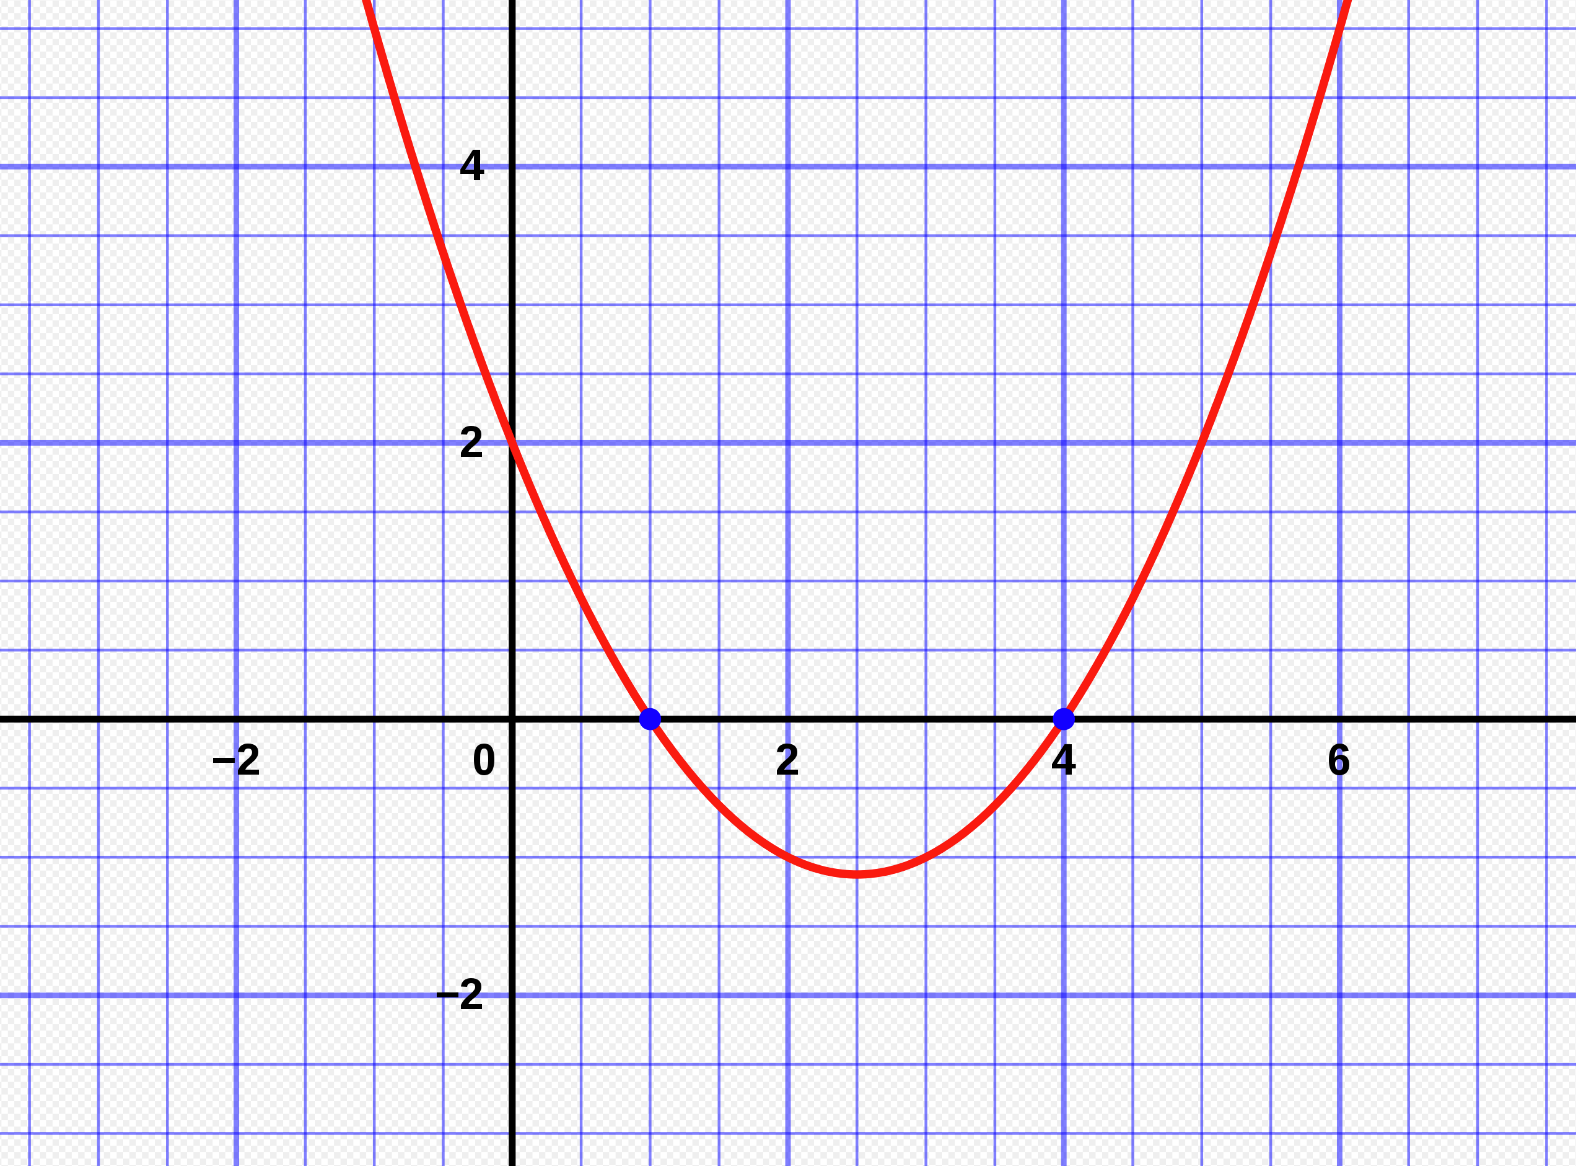
\includegraphics[scale=.15]{quad_equ.png} 

\begin{description}[labelindent=1cm]
	
	\item[\textbf{\underline{Overview:}}] \hfill \vspace{3mm}\\
	We are going to write a Python program to encrypt and decrypt a secret message. 
	
	\item[\textbf{\underline{System Requirements:}}] \hfill \vspace{0mm}

\begin{itemize}
	\item {\bf Computer}: A computer is required to complete this tutorial. Any OS should work.
	\item {\bf Python:} You can an online Python compiler (\href{https://trinket.io/embed/python3/a5bd54189b}{Trinket Python3}) or a Pyhton compiler of your choice.
\end{itemize}

	\item[\textbf{\underline{Problem Statement:}}] \hfill \vspace{0mm} \\
	{\bf Mode 1: Encryption}
	\begin{itemize}

		\item Given: A readable secret message to encrypt with the Caeser Cipher and the cipher key
		
		\item Find: The encrypted message
		 
	\end{itemize}

	{\bf Mode 2: Decryption}
	\begin{itemize}
		
		\item Given: An encrypted secret message to decrypt with the Caeser Cipher and the cipher key
		
		\item Find: The ndecrypted message in a readable format
		
	\end{itemize}

\item[\textbf{\underline{Program Minimum Requirements:}}] \hfill \vspace{0mm}

The program should accomplish the following tasks. 

{\bf Mode 1: Encryption}
\begin{itemize}

	\item The readable message should be stored as an array of characters.

	\item Your program should print readable the message to the screen in character format.
	
	\item Your program should encrypt the message using the Ceaser Cipher (shift each letter in alphabet by the key)
	
	\item Your program should print the encrypted message to the screen.
	
\end{itemize}
	 
{\bf Mode 2: Encryption}
\begin{itemize}
	
	\item The encrypted message name should be stored as an array of characters.
	
	\item Your program should print the encrypted message to the screen in character format.
	
	\item Your program should decrypt the message using the Ceaser Cipher (shift each letter back in alphabet by the key)
	
	\item Your program should print the decrypted message to the screen.
	
\end{itemize}	
\newpage

%\item[\textbf{\underline{Example Code:}}] \hfill \vspace{0mm}
%\begin{enumerate}
%    \item This is the C style way to output text.
%	%\begin{minted}{cpp}
%	\begin{lstlisting}
%
%// Arrays of Characters - GSET - Summer 2021 
%	
%#include <iostream>
%
%using namespace std;
%
%int main()
%{
%
%	char myname[]={"Tristan"};
%	
%	char c = 'T';
%	
%	cout<<"Hello World\n";
%	
%	cout<<myname<<endl; 
%	
%	cout<<myname[1]<<endl;
%	
%	cout<<(int)c<<"\a" <<endl; 
%	
%	return 0;
%}
%
%
%	\end{lstlisting}
%	%\end{minted}
%		
%\end{enumerate}

	\item[\textbf{\underline{Part 3 - Testing:}}] \hfill \vspace{0mm}
	\begin{enumerate}
	
		\item Complete the C++ code to the solve the problem described. \\\\
		
		\item Test your code with different inputs. Is the answer correct? How do you know? Are there certain inputs that do not work? \\\\
		
	
		\item Save your code with the download button or use copy and paste. You can view and edit the code in any text editor. Also, save a copy of the program output for your tutorial summary. \\\\

	\end{enumerate}

\newpage
\item[\textbf{\underline{Solution Code:}}] \hfill \vspace{0mm}
%
%\begin{lstlisting}
%
%\end{lstlisting}
%
%\item[\textbf{\underline{Tutorial Complete:}}] \hfill \vspace{3mm}\\ 
%	Congratulations, after completing {\it Tutorial 2 - Quadratic Equation}, you have begun learning to program in C++! You are now ready to start learning about more complex data structures and program flow. \\
%

\newpage
\item[\textbf{\underline{Tutorial Summary:}}] \hfill \vspace{3mm}\\ 
Write a brief summary of what you accomplished and what you struggled with the most. 

Include the following items in the summary:
\begin{itemize}

\item a copy of the output of your program
\item a description of what the program does and how to use it

\end{itemize}


%\item[\textbf{\underline{Submission on Teams:}}] \hfill \vspace{3mm}\\ 
%Use the appropriate shared folder on Teams to submit your program and summary. Submit the fol1owing items with your TNTech username in the filenames as shown below. \vspace{0mm}\\
%
%\underline{Files for Tutorial 1 (TNTech Username : twhill21)}
%
%\begin{itemize}
%
%\item Tutorial Summary: \textbf{ twhill21\_summary2.txt}
%
%\item C++ Source Code: \textbf{ twhill21\_tutorial2.cpp}
%
%\end{itemize}


\end{description}
\end{document}

